%!TEX root = /Users/velrok/Dropbox/TheoInf Seminar/Ausarbeitung/Main.tex

\subsection{Syntax} % (fold)
\label{sec:syntax}
Die Syntax der Modal Logik entspricht der der Aussagenlogik mit den Erweiterungen $\square$ und $\Diamond$. 
Wie die Negation sind diese unär, das heißt sie beziehen sich nur auf die ihr folgende Formel. Im Folgenden werden die Zeichen $p, q, r, p_3$ für atomare Formeln verwendet.\cite[S.307f]{huth2004logic}\\
\\
\begin{definition}
	\label{def:syntax}
	Die folgende BNF (Backus Naur Form) beschreibt die Syntax der möglichen multi modal Formeln $\phi$.

	\begin{equation}
		\label{eqn:bnf}
		\phi ::= \bot|\top|p|(\neg\phi)|(\phi\wedge\phi)|(\phi\vee\phi)|(\phi\rightarrow\phi)|
		(\phi\leftrightarrow\phi)|(\square\phi)|(\Diamond\phi)
	\end{equation}
\end{definition}
\cite[S.307]{huth2004logic}
\\
\\
Die Formeln 
\begin{equation}
	(p \wedge \Diamond(p \rightarrow \square \neg r))
\end{equation} 
und 
\begin{equation}
	\square((\Diamond q \wedge \neg r) \rightarrow \square p )	
\end{equation}
sind Beispiele für syntaktisch korrekte Multi-Modal-Logik Formeln. Ihre Parse-Trees sind abgebildet in Abbildung~\ref{fig:mmFormel01}.
Wie auch bei der Aussagenlogik binden die unären Operatoren stärker als die Binären.
Sodass unnötige Klammern weggelassen werden können um die Leserlichkeit zu verbessern.\\
\\
\begin{figure}
	\begin{center}
  	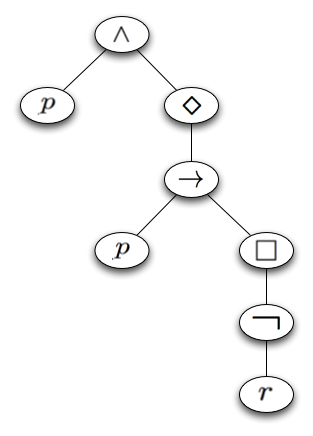
\includegraphics[width=0.4\textwidth]{./Images/mmFormel01.png}
		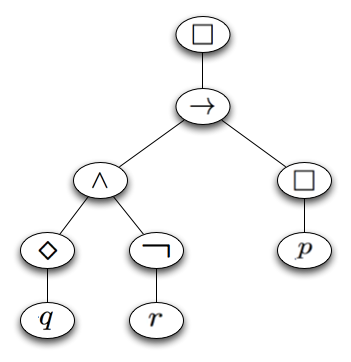
\includegraphics[width=0.4\textwidth]{./Images/mmFormel02.png}
  	\caption{Parse-Tree für $(p \wedge \Diamond(p \rightarrow \square \neg r))$ und 
		$\square((\Diamond q \wedge \neg r) \rightarrow \square p )$}
		\label{fig:mmFormel01}
	\end{center}
\end{figure}
%
Die folgende Liste sortieren die Operatoren nach ihrer Bindungsstärke. 
Beginnend mit den am stärksten bindenden.\\
\begin{itemize}
	\item $\neg, \square, \Diamond$
	\item $\wedge, \vee$
	\item $\rightarrow, \leftrightarrow$
\end{itemize}
%
Im allgemeinen werden die Symbole $\square$ und $\Diamond$ als Box und Raute gelesen. 
Spezifiziert man eine konkrete Logik so werden diese entsprechend ihrer interpretation gelesen. In der Logik für Notwendigkeit wird $\square$ als notwendig und $\Diamond$ als möglich gelesen. In Logik für über das Wissen eines Agenten Q, wird $\square$ als Q weis und $\Diamond$ als soweit Q weis, gelesen.


% section syntax (end)
